%%%%%%%%%%%%%%%%%%%%%%%%%%%%%%%%%%%%%%%%%
% Engineering Calculation Paper
% LaTeX Template
% Version 1.0 (20/1/13)
%
% This template has been downloaded from:
% http://www.LaTeXTemplates.com
%
% Original author:
% Dmitry Volynkin (dim_voly@yahoo.com.au)
%
% License:
% CC BY-NC-SA 3.0 (http://creativecommons.org/licenses/by-nc-sa/3.0/)
%
% Modificaciones por Roberto Cerdas
%
% Si desea utilizar notas al margen, favor leer los comentarios en las líneas 32 y % 52. Si desea colocar un logo, favor leer comentario en línea 54. El comando     % \marginnote{texto} introduce notas al margen.  
%
%%%%%%%%%%%%%%%%%%%%%%%%%%%%%%%%%%%%%%%%%

%----------------------------------------------------------------------------------------
%	PACKAGES AND OTHER DOCUMENT CONFIGURATIONS
%----------------------------------------------------------------------------------------

\documentclass[12pt,a4paper]{article} % Use A4 paper with a 12pt font size - different paper sizes will require manual recalculation of page margins and border positions

\usepackage[spanish]{babel} % Utilizar reglas de idioma español
\usepackage[utf8]{inputenc} % Use UTF-8 encoding
\usepackage{marginnote} % Required for margin notes
\usepackage{wallpaper} % Required to set each page to have a background
\usepackage{lastpage} % Required to print the total number of pages
%\usepackage[left=1.3cm,right=4.6cm,top=1.8cm,bottom=4.0cm,marginparwidth=3.4cm]{geometry} % Comentar la línea abajo y descomentar esta para usar notas al margen
\usepackage[left=1.3cm,right=1.3cm,top=1.8cm,bottom=4.0cm]{geometry} % Adjust page margins
\usepackage{amsmath} % Required for equation customization
\usepackage{amssymb} % Required to include mathematical symbols
\usepackage{xcolor} % Required to specify colors by name
\usepackage[square, comma, sort&compress]{natbib} % Use the natbib reference package - read up on this to edit the reference style; if you want text (e.g. Smith et al., 2012) for the in-text references (instead of numbers), remove 'numbers' 

\usepackage{fancyhdr} % Required to customize headers
\setlength{\headheight}{80pt} % Increase the size of the header to accommodate meta-information
\pagestyle{fancy}\fancyhf{} % Use the custom header specified below
\renewcommand{\headrulewidth}{0pt} % Remove the default horizontal rule under the header

\setlength{\parindent}{0cm} % Remove paragraph indentation
\newcommand{\tab}{\hspace*{2em}} % Defines a new command for some horizontal space

\newcommand\BackgroundStructure{ % Command to specify the background of each page
\setlength{\unitlength}{1mm} % Set the unit length to millimeters

\setlength\fboxsep{0mm} % Adjusts the distance between the frameboxes and the borderlines
\setlength\fboxrule{0.5mm} % Increase the thickness of the border line
\put(10, 10){\fcolorbox{black}{white!10}{\framebox(192,247){}}} % Main content box
%\put(165, 10){\fcolorbox{black}{blue!10}{\framebox(37,247){}}} % Margin box: Descomentar para utilizar notas al margen.
\put(10, 262){\fcolorbox{black}{white!10}{\framebox(192, 25){}}} % Header box
%\put(143, 263){\includegraphics[height=23mm,keepaspectratio]{logo}} % Logo box - maximum height/width: 25x42. Descomentar esta línea para usar logo.
}

%----------------------------------------------------------------------------------------
%	HEADER INFORMATION
%----------------------------------------------------------------------------------------

\fancyhead[L]{\begin{tabular}{l r | l r} % The header is a table with 4 columns
\textbf{Proyecto} & Diseño inversor CMOS & \textbf{Página} & \thepage/\pageref{LastPage} \\ % Project name and page count
\textbf{Trabajo} & Análisis estático y dinámico & \textbf{Actualizado en:} & 25/09/2015 \\ % Job number and last updated date
\textbf{Curso} & VLSI & \textbf{Revisado en:} & 18/09/2015 \\ % Version and reviewed date
\textbf{Diseñador} & López F. - Quirós.J.& \textbf{Revisado por:} & Alfonso Chacón Rodríguez \\ % Designer and reviewer
\end{tabular}}

%----------------------------------------------------------------------------------------

\begin{document}

\AddToShipoutPicture{\BackgroundStructure} % Set the background of each page to that specified above in the header information section

%----------------------------------------------------------------------------------------
%	DOCUMENT CONTENT
%----------------------------------------------------------------------------------------


\section{Resumen} 

En este documento se encontrará el proceso de diseño de un inversor CMOS de tamaño mínimo en la tecnología \textit{ON-semiconductor 0.5}, en el cual se dimensionará el \textit{PMOS} de acuerdo a un análisis estático(misma corriente en los transistores con tensión de inversion igual a la mitad de la alimentación) y a un análisis dinámico (menor tiempo de retardo en los tiempos de levantamiento y caída). También se harán los cálculos para encontrar la resistencia equivalente de los transistores \textit{NMOS} y \textit{PMOS} para la misma tecnología.

\section{Introducción} 

Para el diseño del \textit{PMOS} del inversor, se considera el diseño del \textit{NMOS} segun los parametros minimos del ancho y largo de canal (4$\lambda$/2$\lambda$) en una tecnología \textit{ON-semiconductor 0.5}. Para encontrar la relación que debe tener el ancho de canal \textit{PMOS} con respecto al \textit{NMOS}, se tomarán en cuenta dos diferentes tipos de análisis:\\*
\\*El análisis estático el cual se busca que la corriente de \textit{NMOS} y el \textit{PMOS} sea simétrica. Esto se observa en que la tensión de umbral del inversor sea la mitad de la tensión de alimentación del mismo.\\*
\\*Para este análisis se plantean usar las ecuaciones de \textit{Shockley} para la corriente de un transistor \textit{CMOS}. Esto con el fin de graficar el comportamiento ideal de un transmisor y encontrar la relación de ancho de canal entre los transitores \textit{PMOS} y \textit{NMOS}.

\begin{equation}\label{eqn:NMOS_corte}
I_{dsn}=0
\end{equation}

\begin{equation}\label{eqn:NMOS_lineal}
I_{dsn}=\beta_{n}*(w_{n}/l_{n})*((2*V_{GTn})-V_{dsn})*V_{dsn}
\end{equation}

\begin{equation}\label{eqn:NMOS_sat}
I_{dsn}=\beta_{n}*(w_{n}/l_{n})*(V_{GTn})^2
\end{equation}

El análisis dinámico, se dimensionará el ancho de canal del \textit{PMOS} de tal forma que el tiempo que le toma al inversor pasar de un estado lógico a otro sea el menor posible, siempre y cuando el tiempo que toma de subida y bajada de nivel lógico sean simétricos.

\section{Resultados experimentales}


\subsection{Dimensionamiento de Transistor PMOS}

\subsubsection{Análisis estático}


Para este análisis, primero se realizó una simulación en la plataforma de programación para cálculos matemáticos \textit{Octave}, esto con el fin de tener una aproximación de la relación que debe tener el ancho de canal del \textit{PMOS} con el \textit{NMOS} para que la tensión de umbral del inversor $V_{inv}=V_{dd}/2$. Se utilizaron las ecuaciones en región de corte (Ec.[\ref{eqn:NMOS_corte}]), lineal (Ec.[\ref{eqn:NMOS_lineal}]) y saturación (Ec.[\ref{eqn:NMOS_sat}]) y conociendo que para ciertos rangos de valores de tensión de entrada, los transistores se encontraban en regiones de polarización específicas y la tensión de salida tenia un comportamiento particular como se muestra en la tabla \ref{table:Tabla_polarizacion}.\\*
\\*

\begin{table}\label{table:Tabla_polarizacion}
\begin{center}
\begin{tabular}{c||c||c||c}
Numero & Rango entrada & Región PMOS & Región NMOS\\
\hline
\hline
1 & $V_{in}<V_{tn}$ & Lineal & Corte \\
2 & $V_{tn}<=V_{in}<V_{inv}$ & Lineal & Saturación \\
3 & $V_{in}=V_{inv}$ & Saturación & Saturación\\
4 & $V_{inv}<V_{in}<=V_{dd}+V_{tp}$ & Saturación & Lineal\\
5 & $V_{in}>V_{dd}+V_{tp}$ & Corte & Lineal\\
\hline
\end{tabular}
\caption{Regiones inversor CMOS Vin vs Vout}
\end{center}
\end{table}

El análisis que se realizo con el software \textit{Octave} arrojo la gráfica que se muestra en la fig.\ref{fig:inv_est}, la cual dio como resultado que la relación de $\beta$ es de r=4, lo cual significa que el transistor \textit{PMOS} debe de ser 4 veces más ancho que el \textit{NMOS} para que las regiones sean simétricas.\\*

\begin{figure}[htbp]
  \centering
    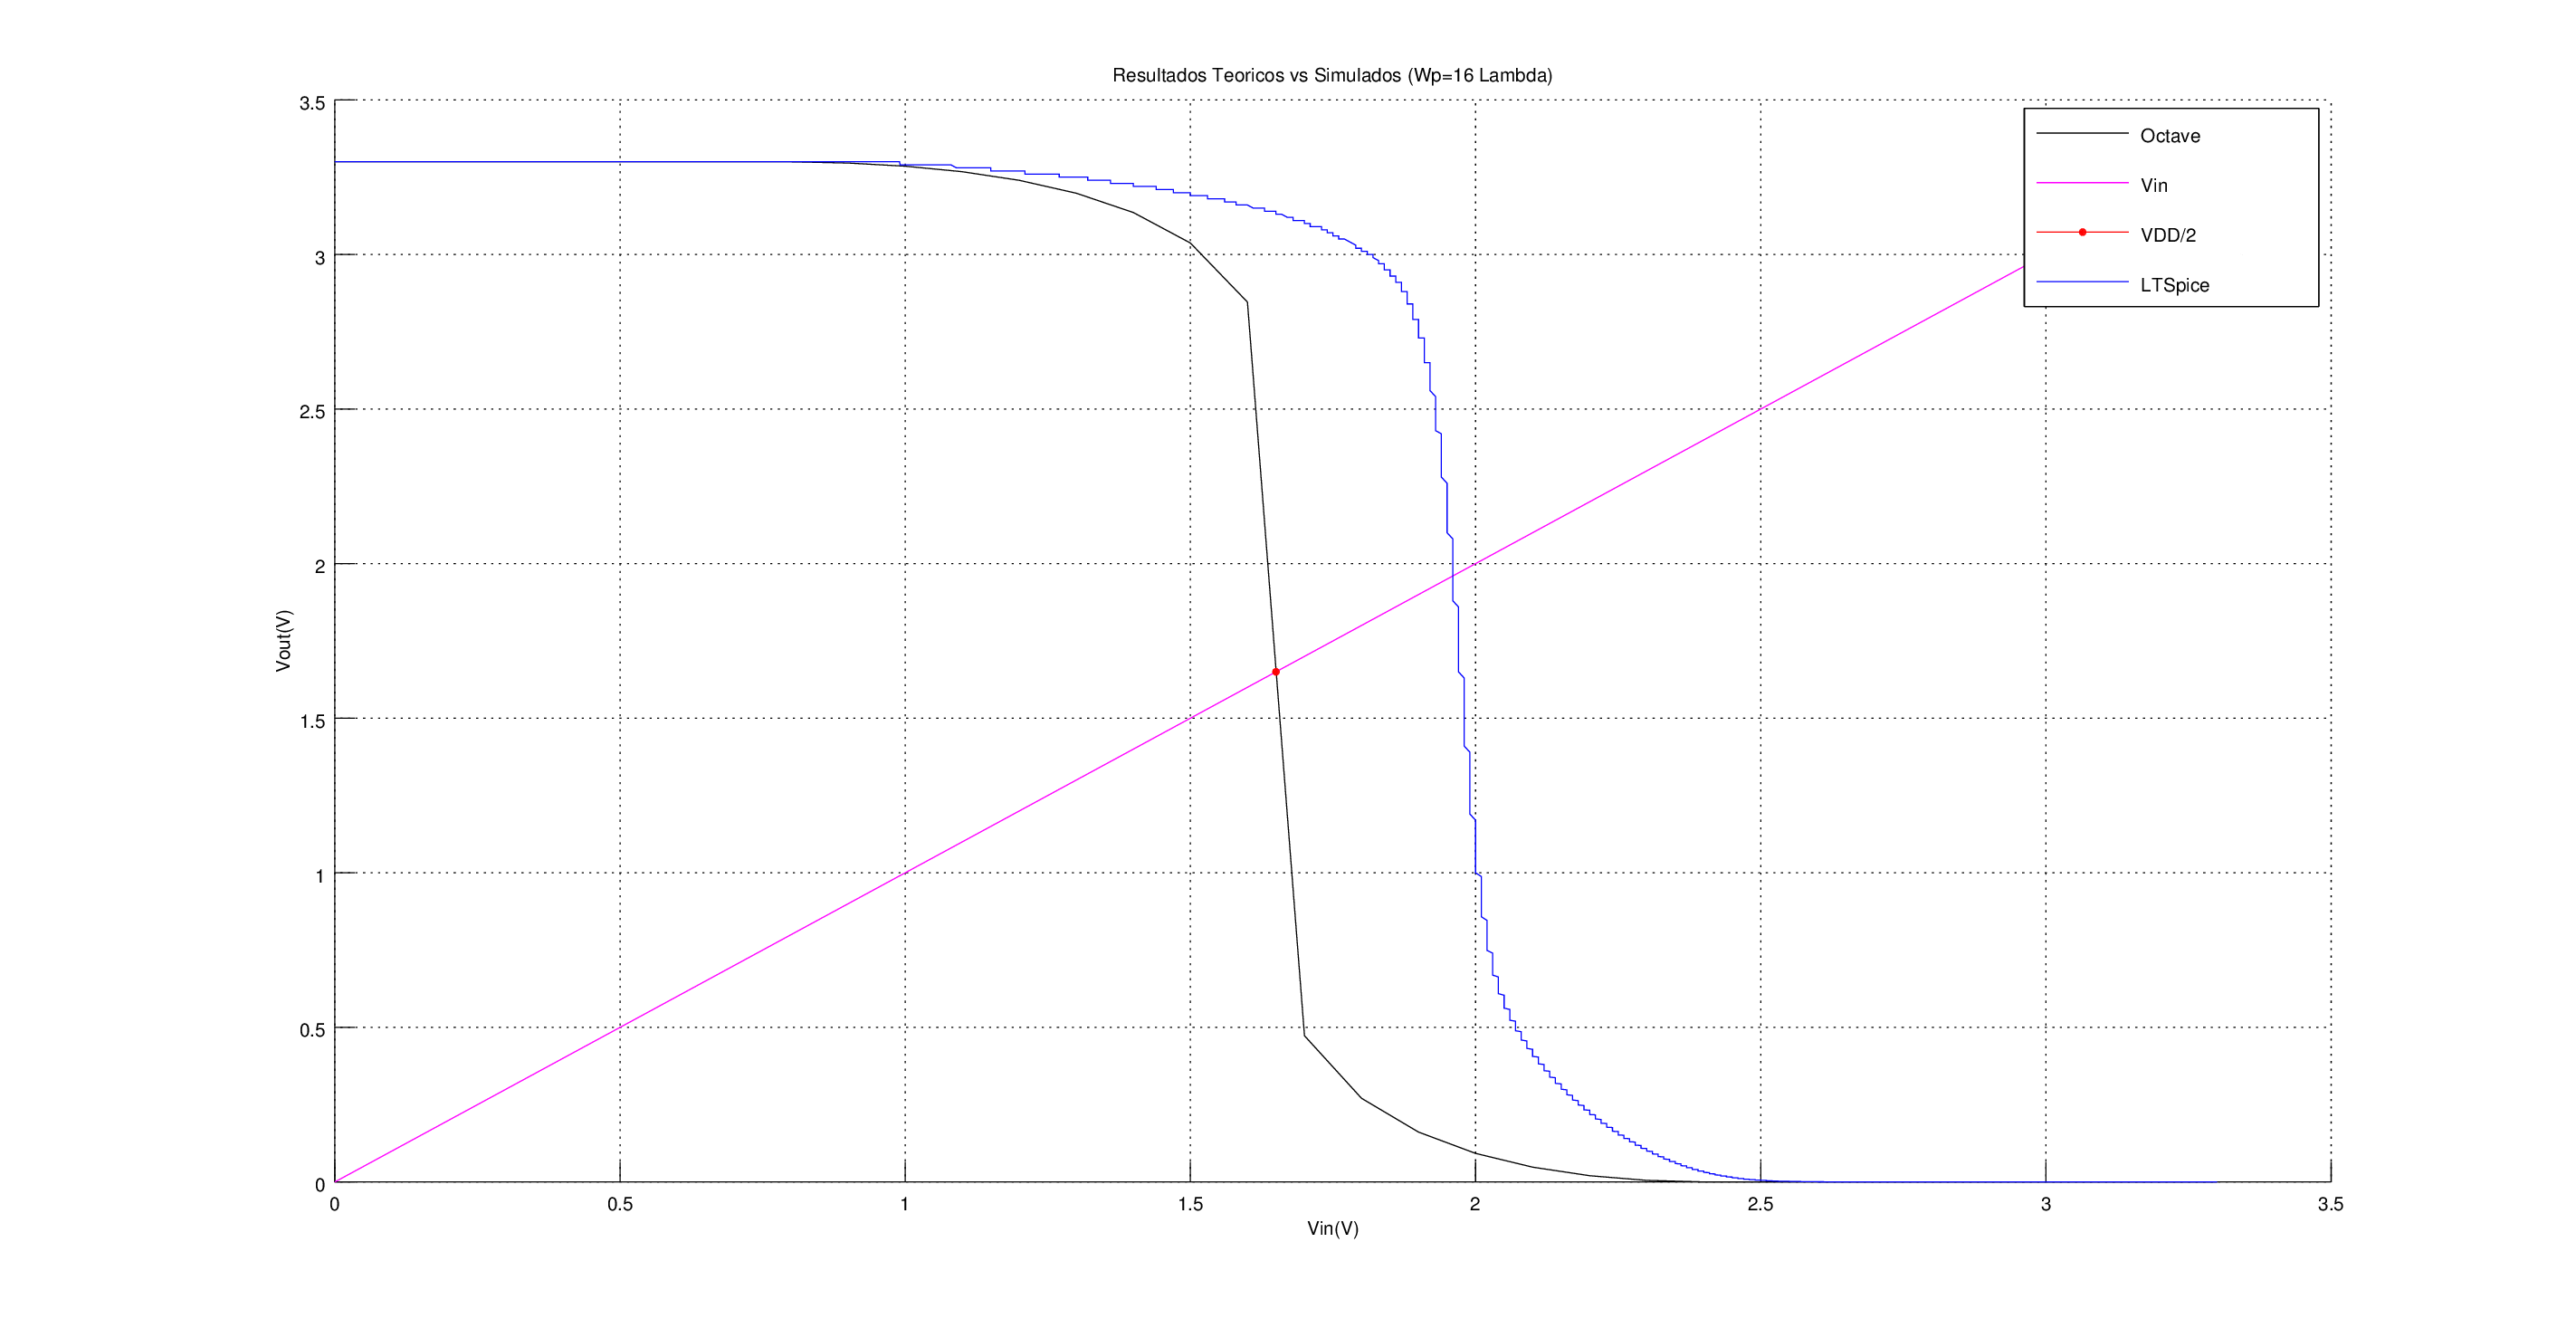
\includegraphics[scale=0.2]{./Inv_16lam.png}
    \rule{35em}{0.5pt}
  \caption[IdealvsSim]{Graficas \textit{Octate} Ideal vs Simulacion \textit{Electric}}
  \label{fig:inv_est}
\end{figure}

Para la simulación experimental, se usó el programa \textit{Electric}. En esta simulación se utilizó el archivo \textit{Mosis\_5} para las constantes de la tecnología MOSIS 0.5. Ya realizada la simulación del inversor (fig.\ref{fig:inv_est2}) con la relación de ancho de canal calculado anteriormente encontramos que la proporción de regiones en el inversor no es la esperada, por lo que se decidió volver a dimensionar el ancho de los canales con respecto a las simulaciones y encontramos que de manera experimental la relación correcta es \textit{r=1.575}. 


\begin{figure}[htbp]
  \centering
    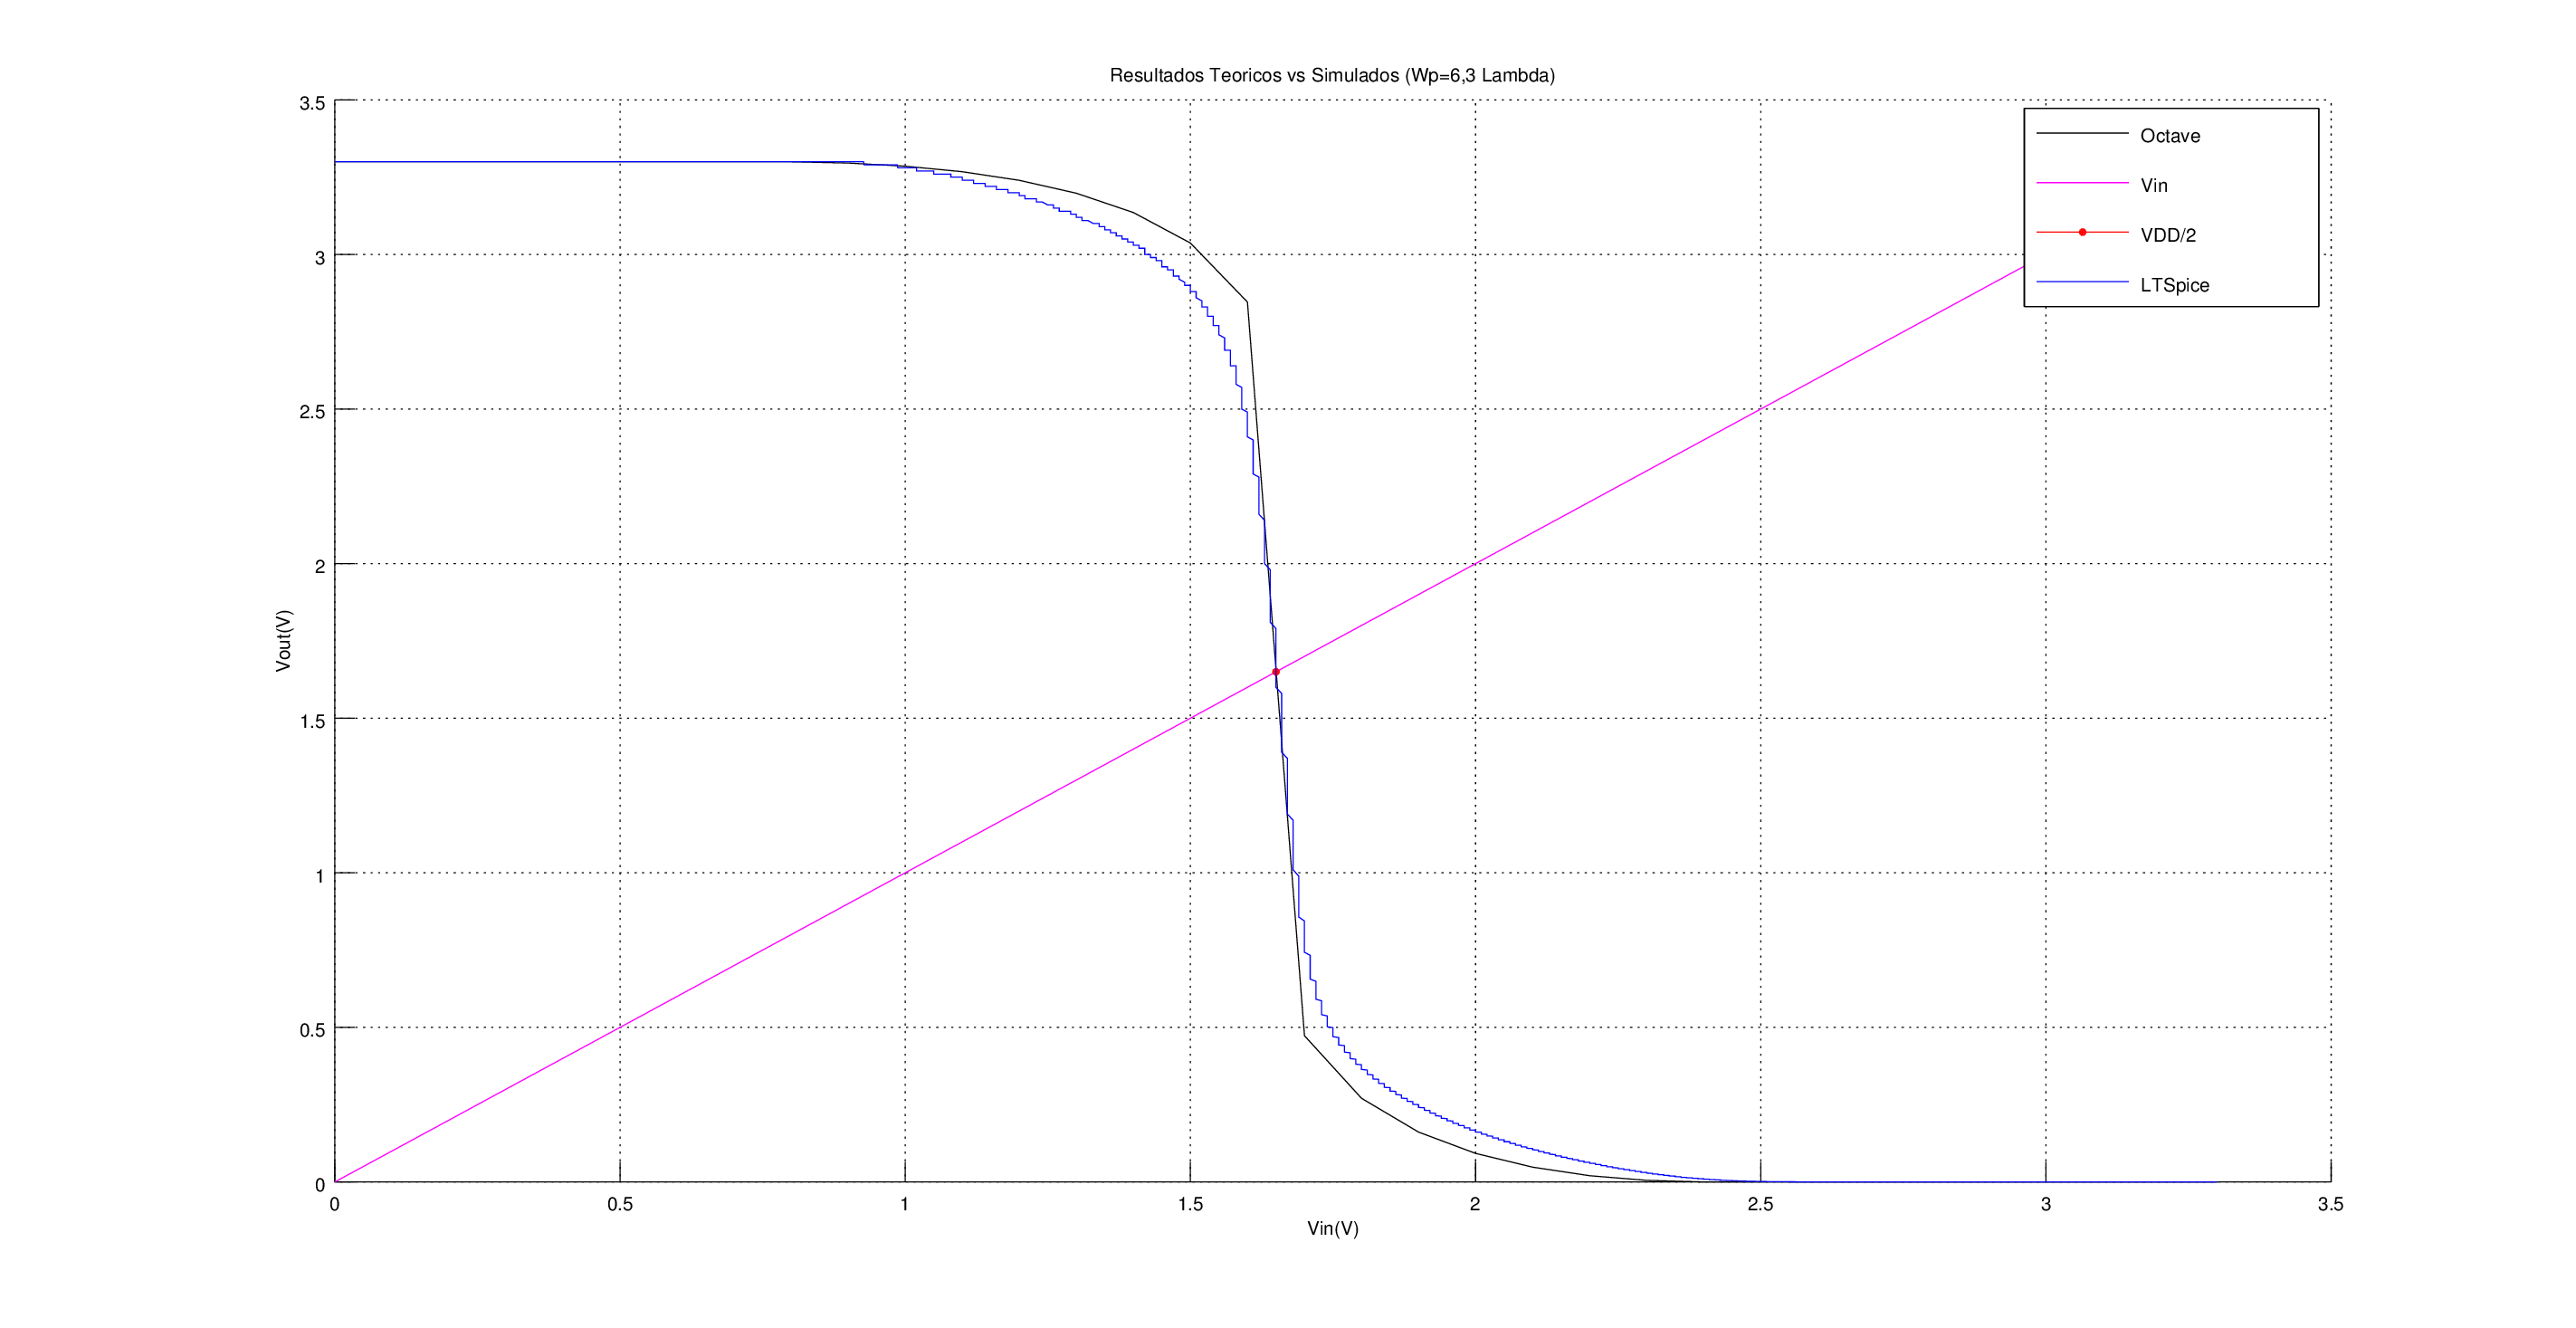
\includegraphics[scale=0.2]{./Inv_63lam.png}
    \rule{35em}{0.5pt}
  \caption[IdealvsSim]{Graficas \textit{Octate} Ideal vs Simulación Ajustada \textit{Electric}}
  \label{fig:inv_est2}
\end{figure}


\subsubsection{Análisis Dinámico.}

En este método se determina  el valor del ancho de canal del transistor \textit{PMOS}, de manera que el tiempo de propagación sea mínimo, y que los tiempos de propagación de la señal de alto a bajo y viceversa sean simétricos, suponiendo que el inversor tiene una carga conectada igual así mismo. Se debe tener en consideración que aumentar el ancho del canal en el transistor \textit{PMOS} mejora el parámetro $\textit{t}_\textit{plh}$, pero también degrada el $\textit{t}_\textit{phl}$, esto debido a que aumenta la corriente de carga en el carga en el transitor, pero tambień aumenta el valor de las capacitancias parásitas del dispositivo.\\

Para obtener una relacion óptima de tamaños entre el \textit{PMOS} y el \textit{NMOS} que permita mejorar el retardo de propagación de subida y bajada, se utiliza la siguiente formula:

\begin{equation}\label{eqn:Beta}
\beta= \sqrt{r} 
\end{equation}

\begin{equation}\label{eqn:r}
r= \frac{Req_P}{Req_N}
\end{equation}
 
Los valores de resistencia utilizados para calcular $\beta$, son los calculados en el apartado 2 de esta tarea, específicamente del método de variación del \textit{fanout}, esto debido a que con este método se obtienen valores más cercanos a los esperados. De la ecuación  se obtiene que:

\begin{equation}\label{eqn:Beta2}
\beta= \sqrt{\frac{15.375k\Omega}{9.0k\Omega}} = 1.3070
\end{equation}

Y sabiedo que:

\begin{equation}\label{eqn:Beta3}
\beta= \frac{(\frac{W}{l})_P}{(\frac{W}{l})_N} 
\end{equation}

\begin{equation}\label{eqn:Beta4}
\beta= \frac{W_P}{W_N} 
\end{equation}

\begin{equation}\label{eqn:Beta5}
W_P= 1.3070*W_N = 5\lambda  
\end{equation}\\

Tambień se calculan los tiempos teóricos de de propagación del inversor, mediante el modelo de \textit{delay RC} aplicado al inversor.

\begin{equation}\label{eqn:DelayRC2}
t_{plh} = 0.69*Req_P*C_L = 15.38ps
\end{equation}

\begin{equation}\label{eqn:DelayRC}
t_{phl} = 0.69*Req_N*C_L = 9.00ps
\end{equation}\\

Con el tamaño del ancho del canal del \textit{PMOS} calculado, se procede a simular el circuito que se muestra en la fig.\ref{fig:Inversor_1b} haciendo uso de los software \textit{ELectric} y \textit{LTSpice}, para poder encontrar los tiempos de propagación.\\

\begin{figure}[htbp]
  \centering
    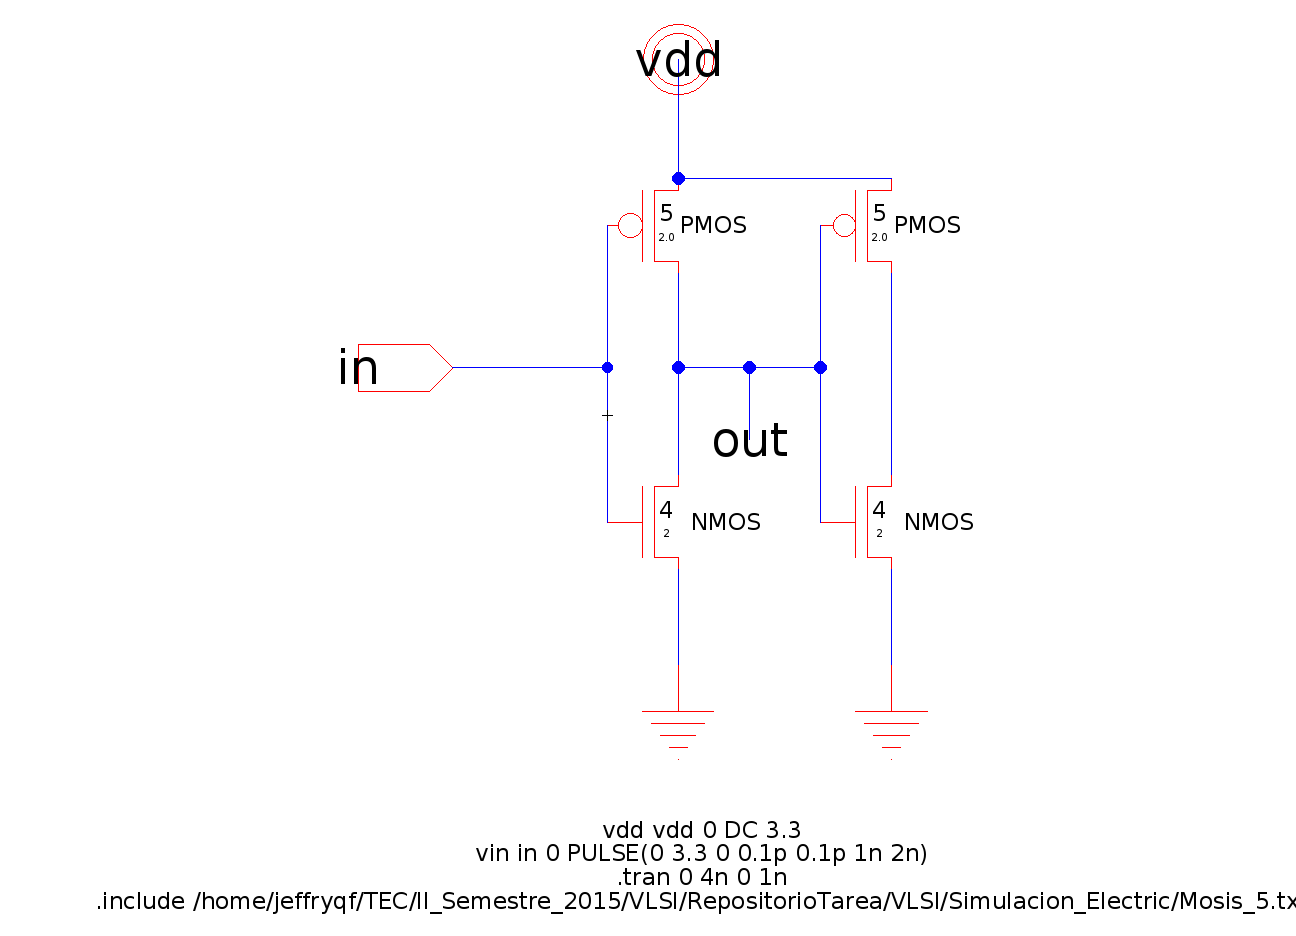
\includegraphics[scale=0.25]{./Inversor_estatico_1b.png}
    \rule{35em}{0.3pt}
  \caption[INV]{Inversor con una carga igual a si mismo.}
  \label{fig:Inversor_1b}
\end{figure}

A partir de la simulación del circuito, se puede observar en la fig.\ref{fig:tLH_tHL}, las gráficas obtenidas en \textit{LTSpice} de los tiempos de propagación de la señal.\\

\begin{figure}[htbp]
  \centering
    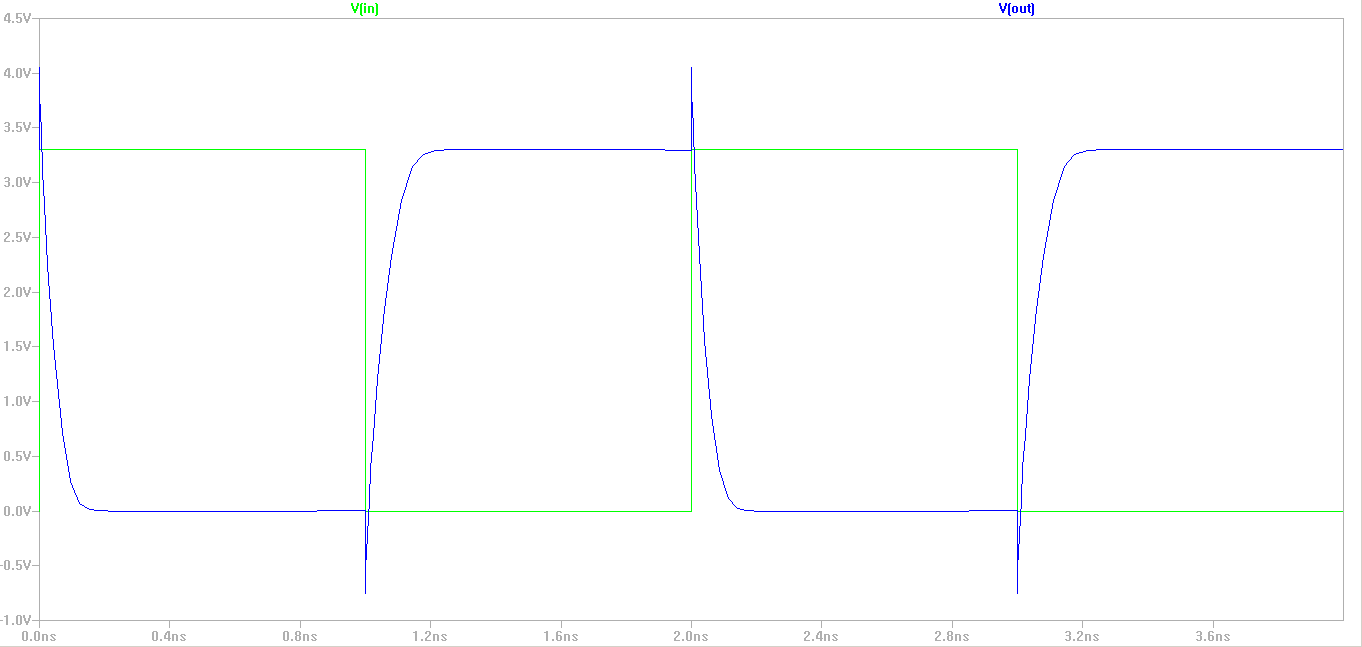
\includegraphics[scale=0.35]{./tLH_tHL.png}
    \rule{35em}{0.3pt}
  \caption[INV2]{Simulación de tiempos de retardo en un inversor.}
  \label{fig:tLH_tHL}
\end{figure}

A partir de esta simulación, y ajustando los valores en \textit{LTSpice}, se obtiene que el ancho apropiado del canal del transistor \textit{PMOS} es de 6$\lambda$, obtiendo con este ajuste los siguientes valores de tiempos de propagación:

\begin{equation}\label{eqn:t_plh}
t_{phl} = 60,8725ps
\end{equation}

\begin{equation}\label{eqn:t_phl}
t_{phl} = 66,273ps
\end{equation}\\

Con estos valores se observa que los tiempos son bastantes cercanos, con una diferencia de \textit{5.4005ps}, dando como resultado que los tiempos de propagación sean bastante simétricos.\\

En contraposición con los valores calculados, los valores experimentales presentan un tiempo de propagacion mayor, pero con un porcentaje de diferencia de apenas un \textit{8\%}, mientras que los valores calculados presentan un porcentaje de diferencia de \textit{70\%}, por lo que los resultados experimentales demuestran ser más simétricos que los teóricos.\\


Con ayuda del software matemático \textit{Octave}, se procede ahora a comparar las curvas de trasferencia que se obtuvieron en este punto, con la obtenida en el punto anterior. Los resultados se observan en la fig.\ref{fig:DC_Comp}.\\


\begin{figure}[htbp]
  \centering
    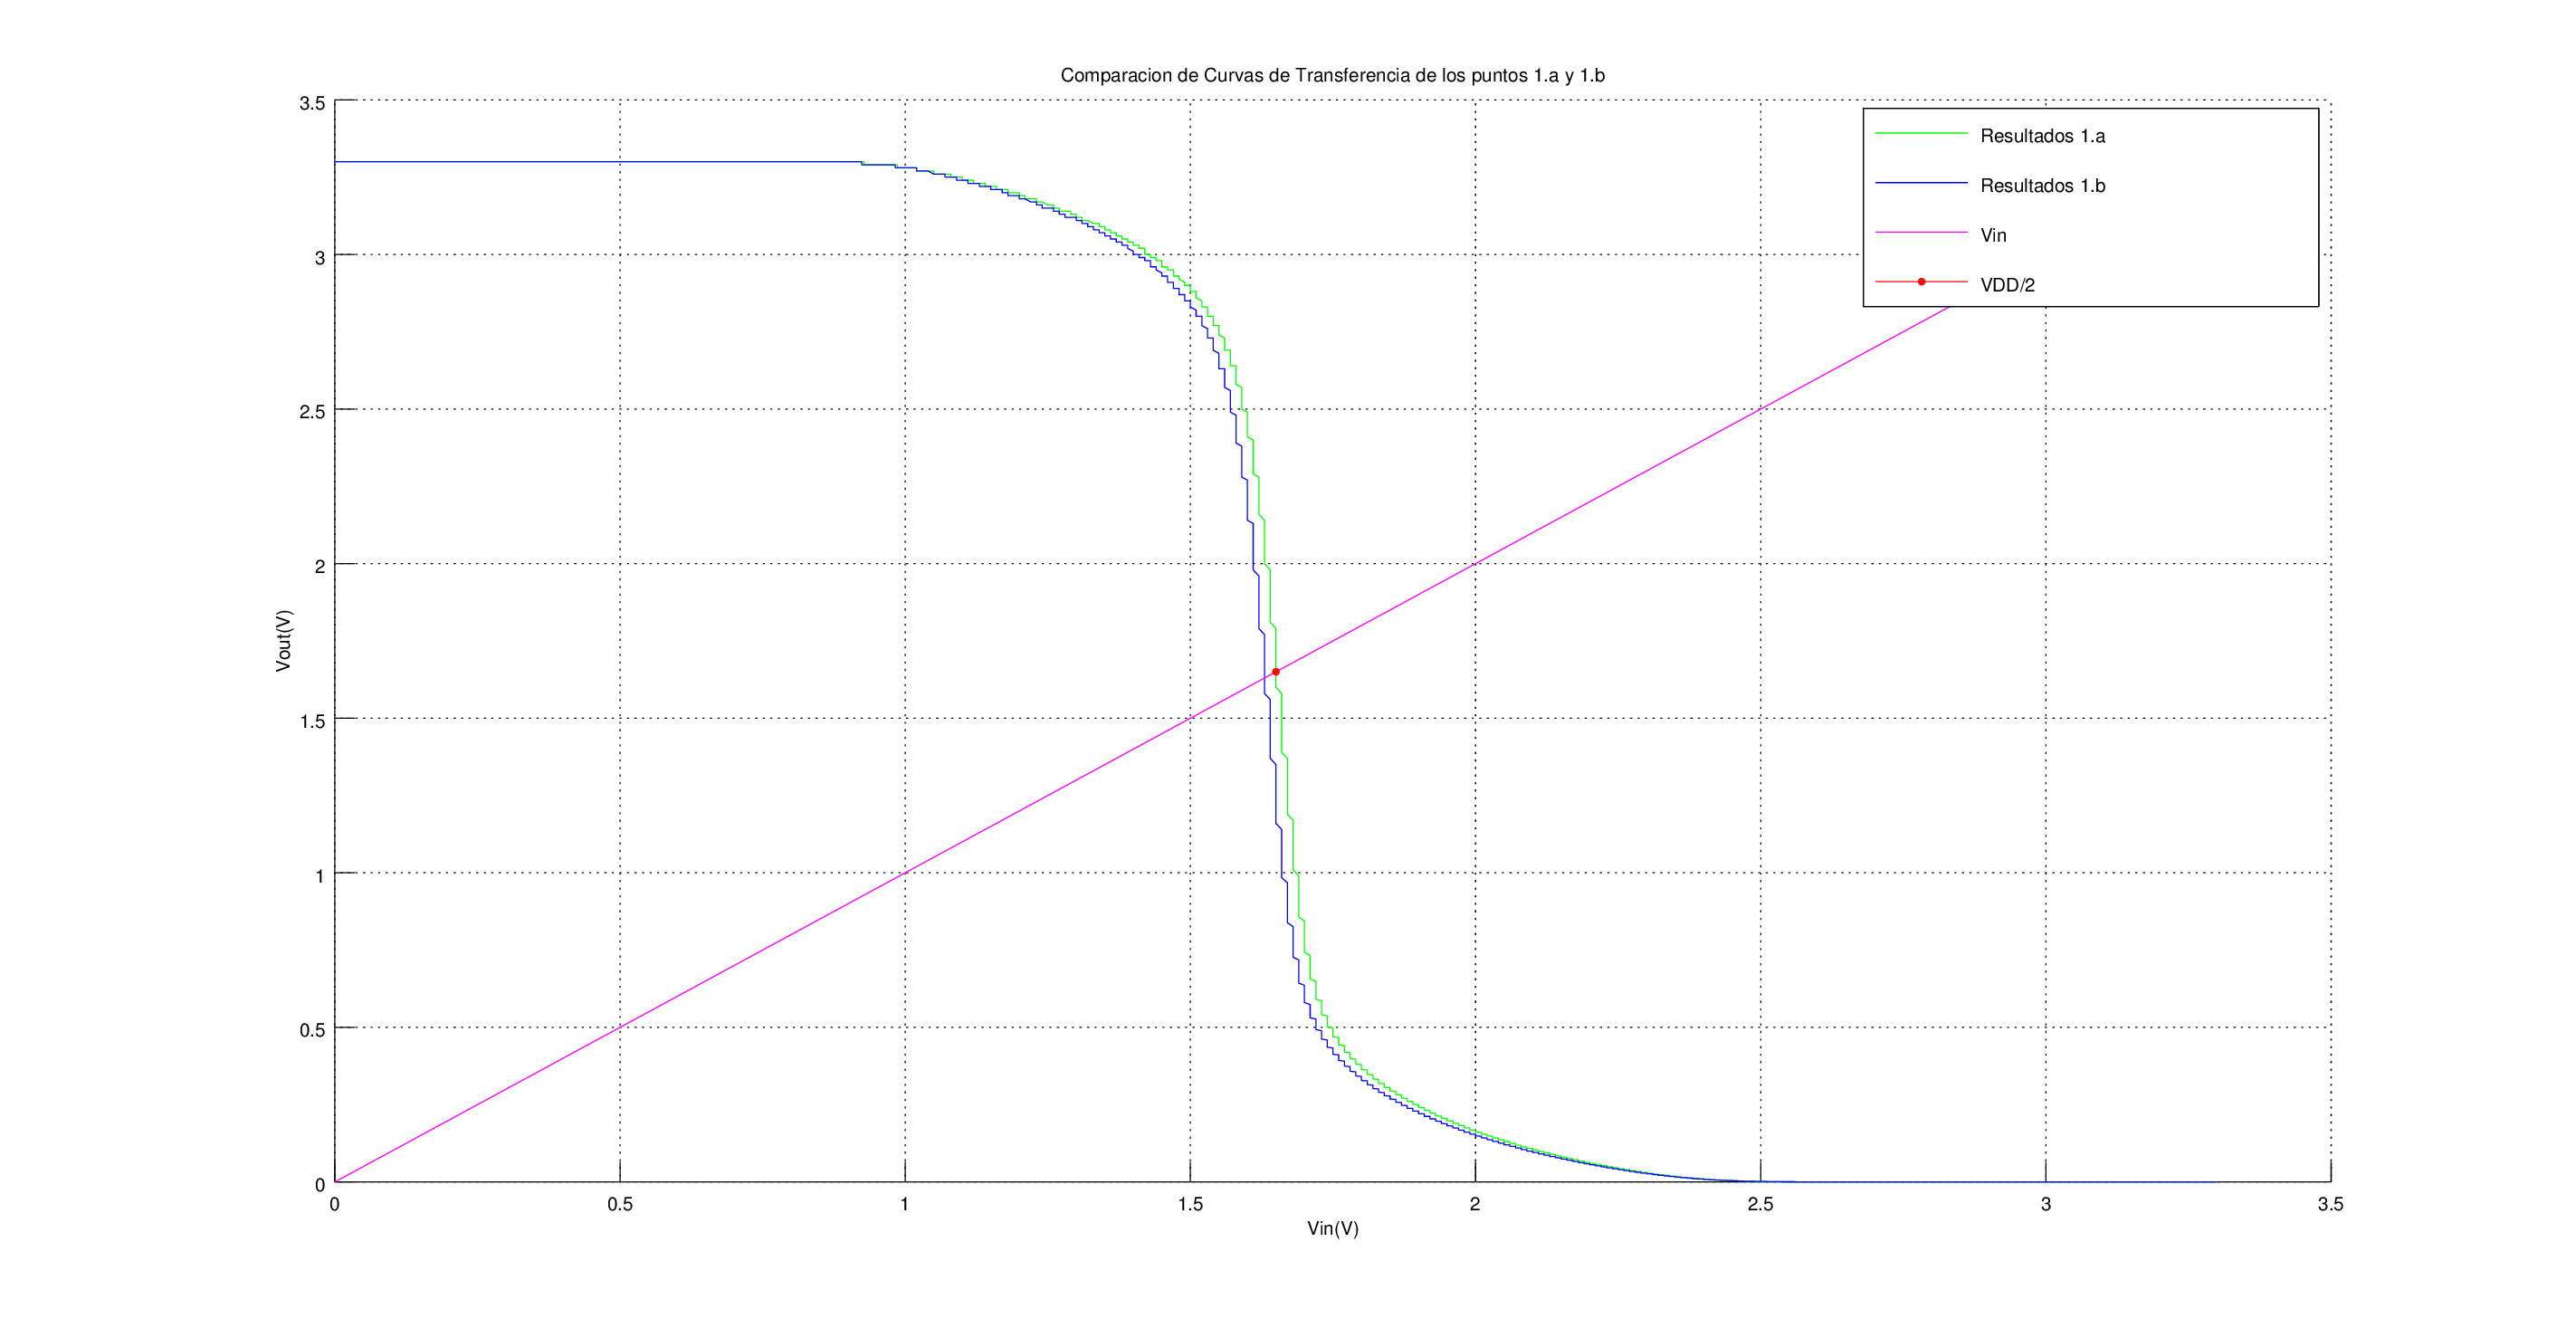
\includegraphics[scale=0.25]{./DC_1a_1b.png}
    \rule{35em}{0.3pt}
  \caption[DCim]{Curvas de transferencia DC obtenidas en el punto 1.a y 1b.}
  \label{fig:DC_Comp}
\end{figure}

En la fig.\ref{fig:DC_Comp} se puede observar que la nueva curva de trasnferencia, de color azul, no tiene una tensión de umbral exactamente en \textit{1.65V}, pero no se aleja demasiado de ese valor, por lo que es una aproximación aceptable. \\

A continuación se procede a comparar las mediciones de las corriente de corto circuito obtenidas en el punto \textit{1.a} y \textit{1.b}, graficando dichas mediciones en \textit{Octave}. En la fig.\ref{fig:CC} se observan las 2 curvas obtenidas transpuestas.

\begin{figure}[htbp]
  \centering
    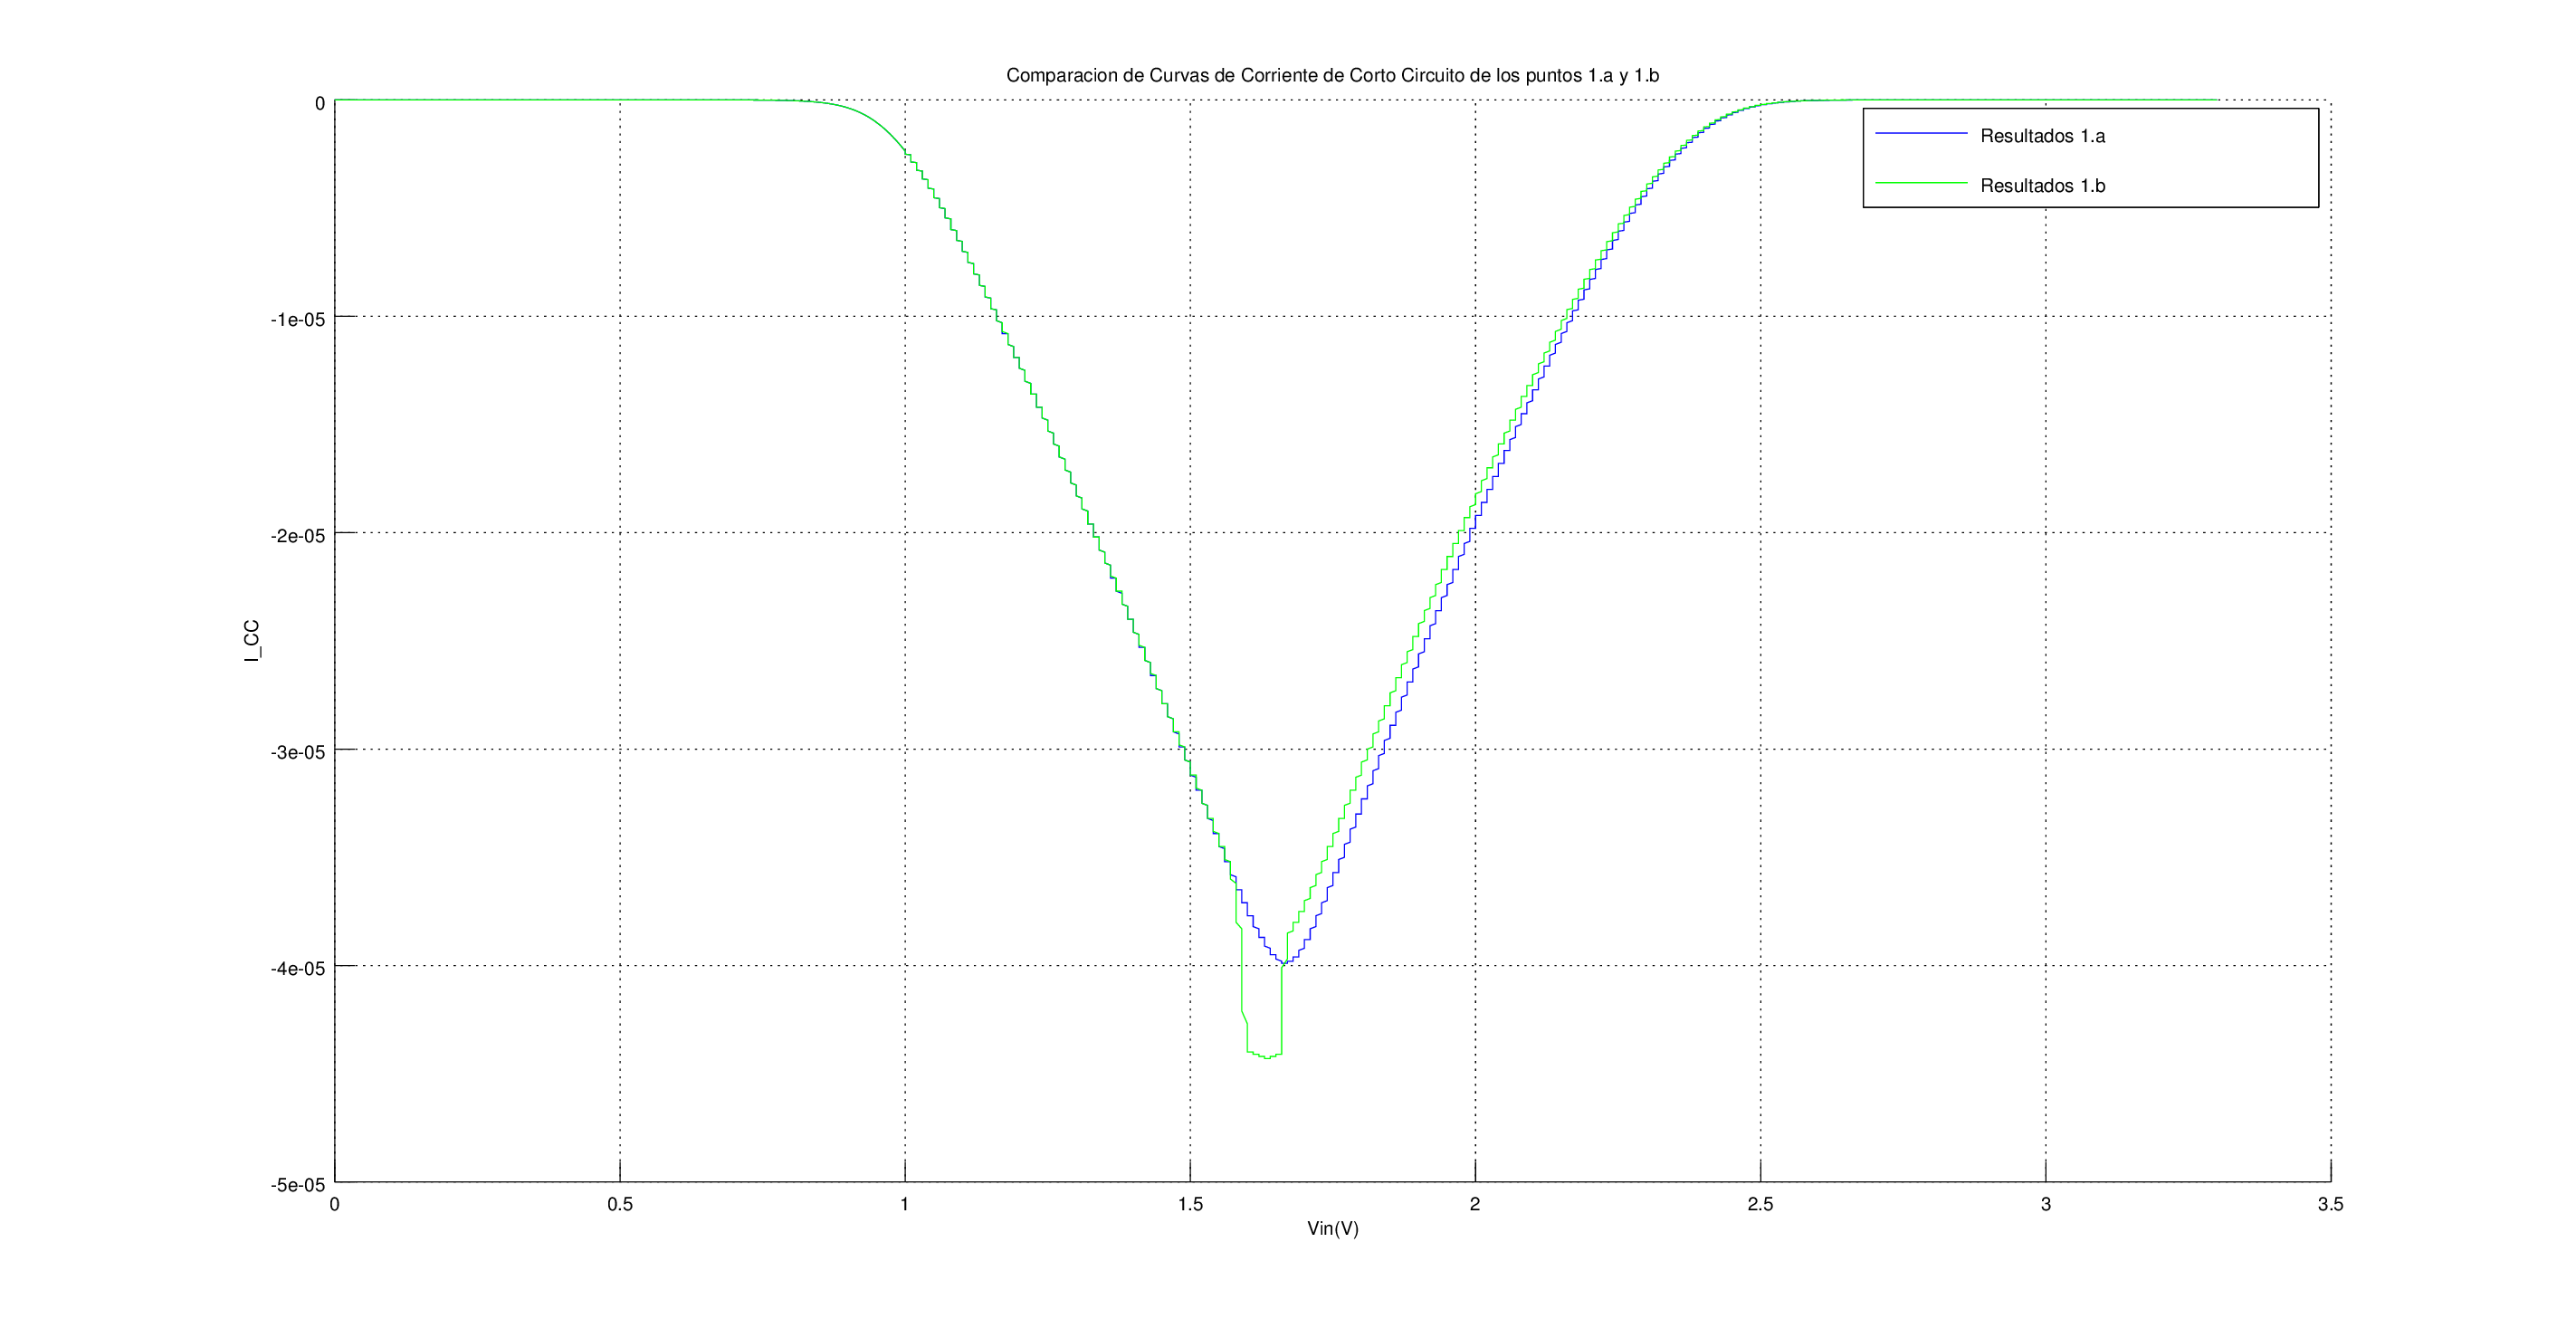
\includegraphics[scale=0.4]{./Comp_Corriente_ICC.png}
    \rule{35em}{0.3pt}
  \caption[CC]{Corriente de Corto Circuito de los puntos \textit{1.a} y \textit{1.b}}
  \label{fig:CC}
\end{figure}


\subsection{Cálculo de Resistencias de Canal}

El cálculo de la resistencia de canal para un transistor \textit{PMOS} y \textit{NMOS} se realizará utilizando dos métodos diferentes.\\

En el primer método se coloca una capacitancia de descarga en paralelo con el transistor \textit{NMOS}, y una de carga en serie con el transistor \textit{PMOS}, con el objetivo de obtener las curvas de comportamiento de la corriente $\textit{I}_{\textit{d}}$, mientras se descarga o carga un capacitor, respectivamente. En el caso de descarga la tensión del \textit{drain} del transistor \textit{NMOS} debera moverse de $\textit{V}_{\textit{DD}}$ $\longrightarrow$ $\textit{V}_{\textit{DD}}/2$. En el caso de carga la tensión del \textit{drain} del transistor \textit{PMOS} debera moverse de $\textit{0}$ $\longrightarrow$ $\textit{V}_{\textit{DD}}/2$.\\

El tamaño de dicha capacitancia debe ser lo suficientemente grande como para despreciar el efecto de las capacitancias parásitas del transistor. Una vez obtenidas las curvas de la corriente, se calcula el promedio de valores de resistencia, mientras la tension se mueve de $\textit{V}_{\textit{DD}}$ $\longrightarrow$ $\textit{V}_{\textit{DD}}/2$ o de $\textit{0}$ $\longrightarrow$ $\textit{V}_{\textit{DD}}/2$, dependiendo del caso.\\

En el segundo método se buscarán los tiempos de levantamiento y caída de los transistores NMOS y PMOS para 2 valores distintos de Fanouts, esto con el objetivo de eliminar de los cálculos las capacitancias parásita que posee en el drain y el cálculo de la resistencia dependa solamente de los diferenciales de tiempos entre los Fanouts y la capacitancia de Gate.

\subsubsection{Carga y descarga de un capacitor}

Para el cálculo de las resistencias de canal de cada transistor, se utilizo una capacitancia de carga y descarga de \textit{1pF}, se montaron los circuitos de las figuras \ref{fig:R_PMOS} y \ref{fig:R_NMOS} en el software \textit{Electric} y se simularon los resultados en  \textit{LTSpice}, obteniendo las curvas que se observan en las figuras \ref{fig:Grafica_R_PMOS} y \ref{fig:Grafica_R_NMOS}, para el caso de carga y descarga, respectivamente.\\

\begin{figure}[htbp]
  \centering
    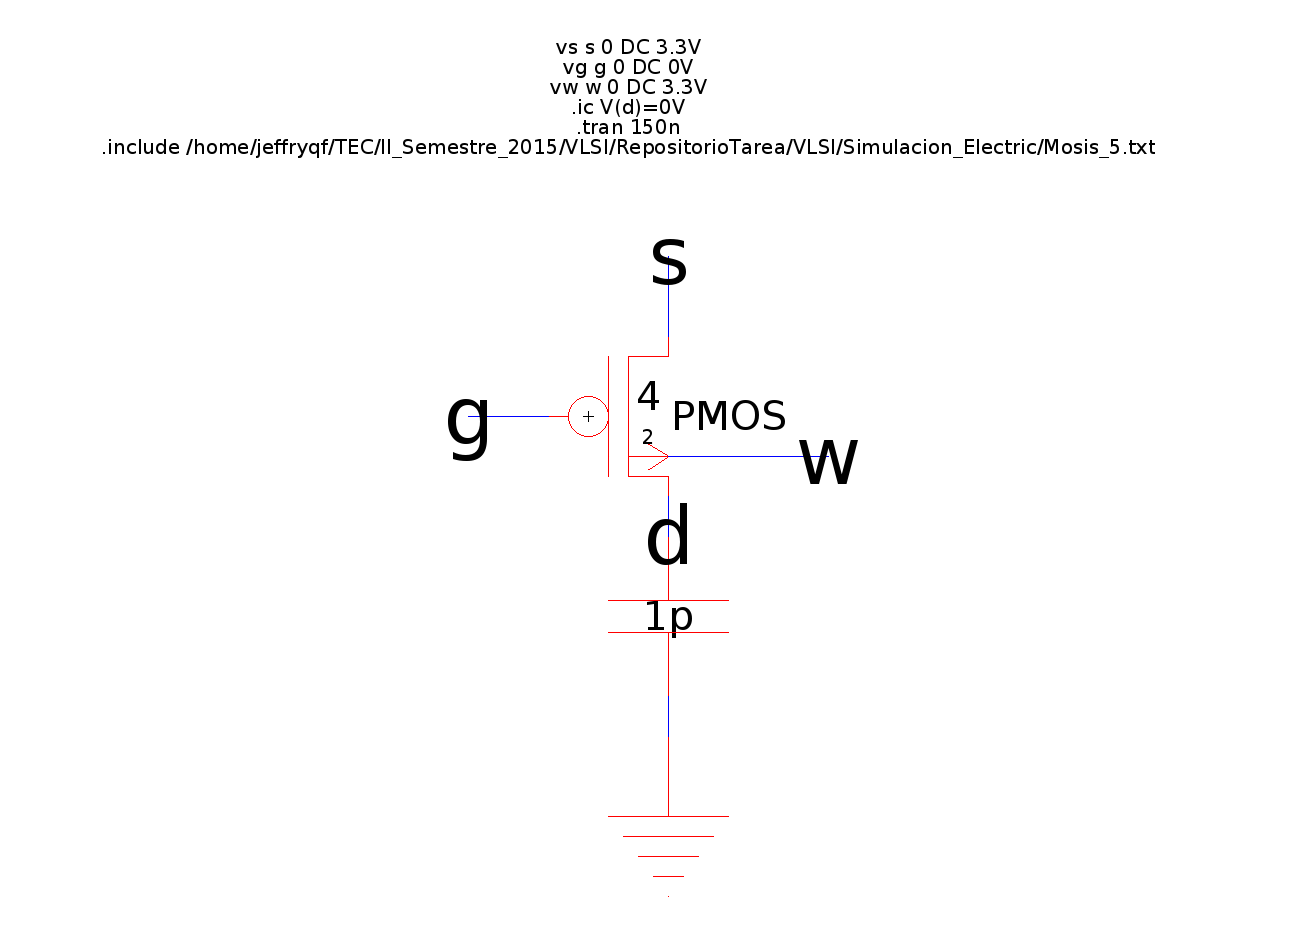
\includegraphics[scale=0.3]{./R_PMOS.png}
    \rule{35em}{0.3pt}
  \caption[C_Carga]{Circuito de Carga de Capacitor.}
  \label{fig:R_PMOS}
\end{figure}

\begin{figure}[htbp]
  \centering
  	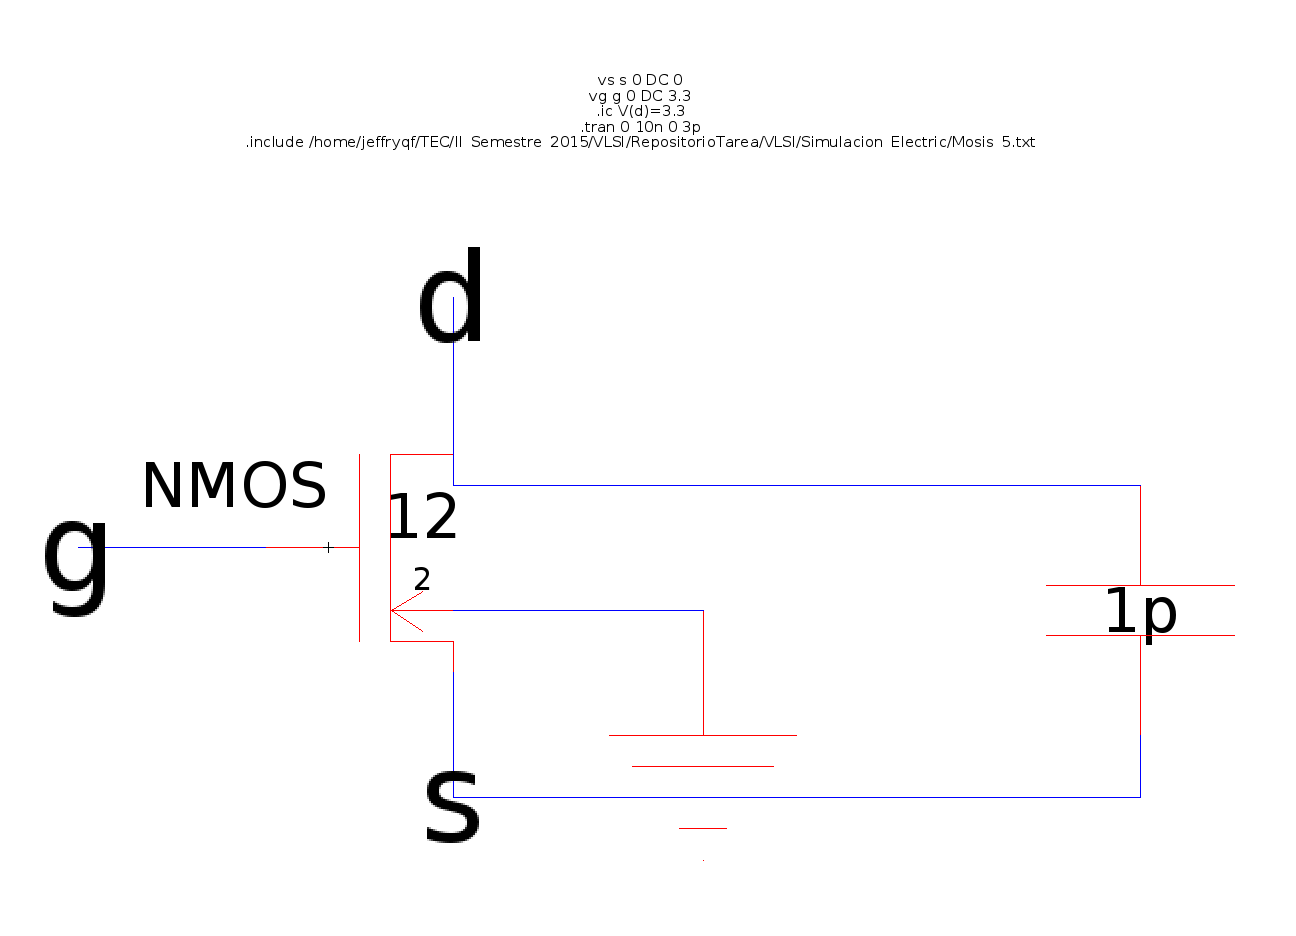
\includegraphics[scale=0.3]{./R_NMOS.png}
    \rule{35em}{0.3pt}
  \caption[C_Descarga]{Circuito de Descarga de Capacitor.}
  \label{fig:R_NMOS}
\end{figure}

\begin{figure}[htbp]
  \centering
    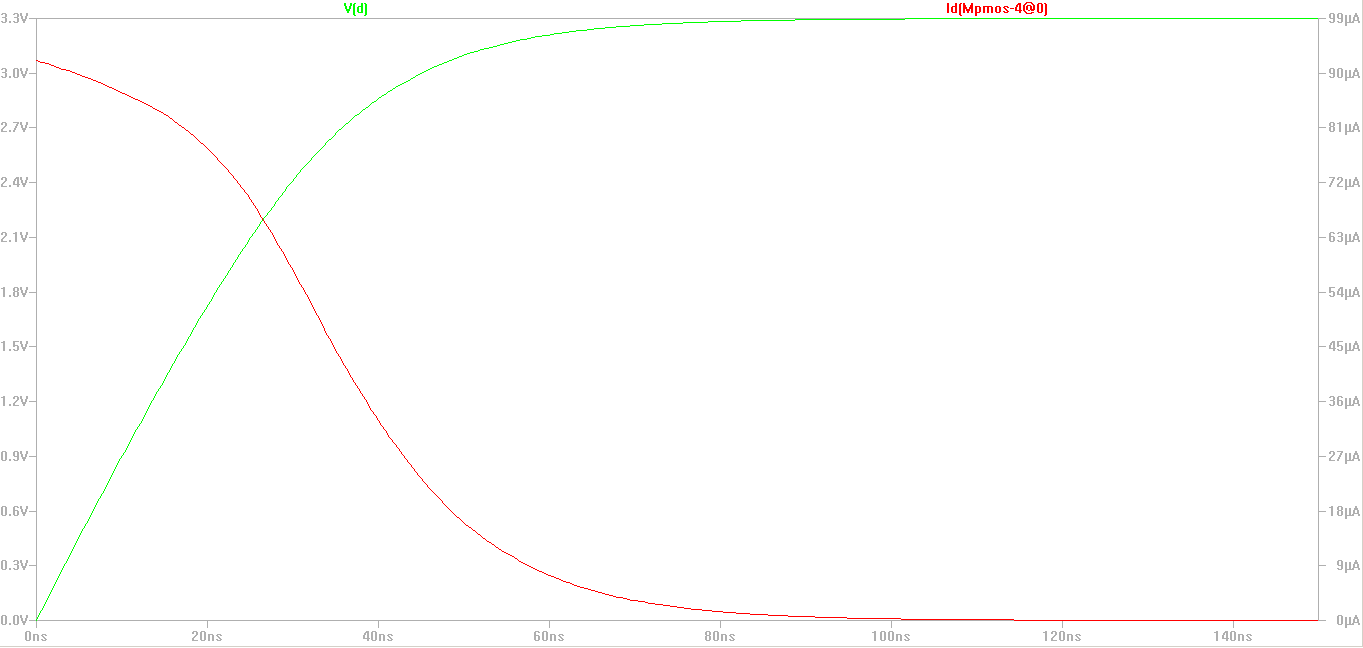
\includegraphics[scale=0.3]{./Grafica_R_PMOS.png}
   \rule{35em}{0.3pt}
  \caption[G_Carga]{Grafica de comportamiento de $\textit{I}_{\textit{d}}$ durante la carga del Capacitor.}
  \label{fig:Grafica_R_PMOS}
\end{figure}

\begin{figure}[htbp]
 \centering
    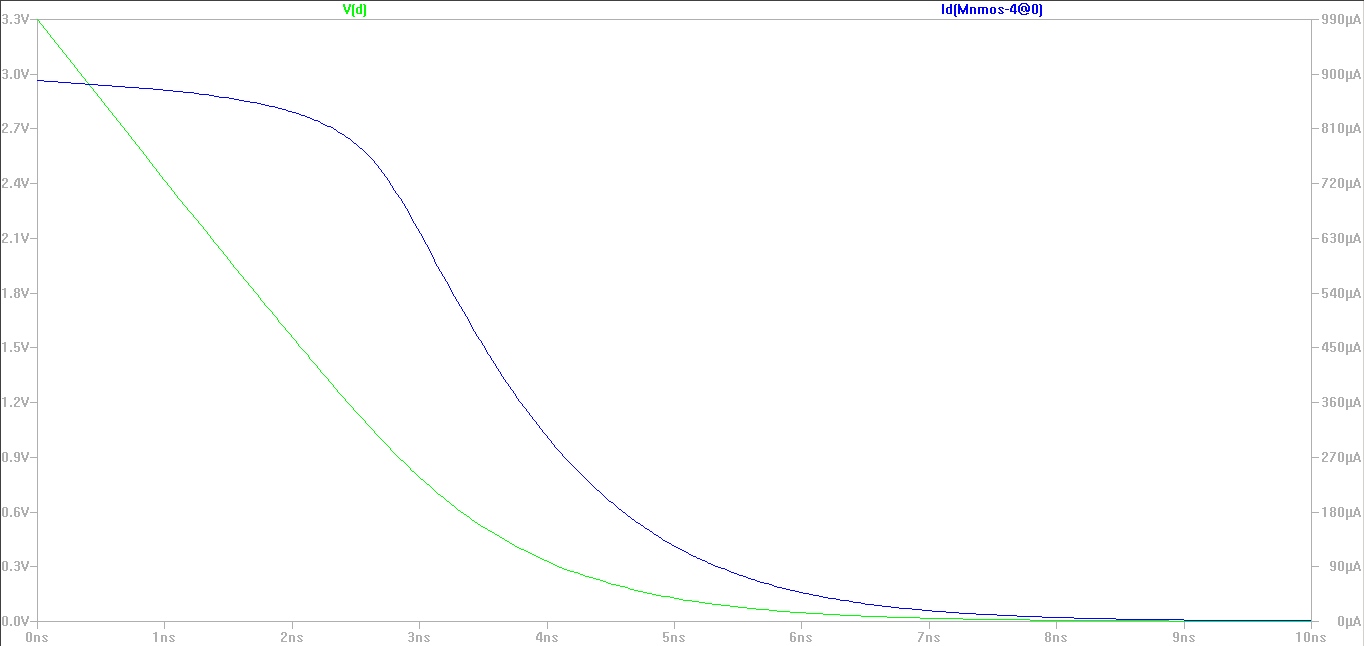
\includegraphics[scale=0.3]{./Grafica_R_NMOS.png}
    \rule{35em}{0.3pt}
  \caption[G_Descarga]{Grafica de comportamiento de $\textit{I}_{\textit{d}}$ durante la descarga del Capacitor.}
  \label{fig:Grafica_R_NMOS}
\end{figure}

Utilizando un pequeño script en \textit{Octave}, se procesan los puntos obtenidos en estas graficas y se calculan la resistencias de canal promedio de cada transistor, obteniendo los siguientes resultados:

\begin{equation}\label{eqn:R_PMOS}
Req_P = 8.7860k\Omega
\end{equation}

\begin{equation}\label{eqn:R_NMOS}
Req_N = 2.6919k\Omega
\end{equation}

\subsubsection{Método de Fanout}

El método de Fanout plantea encontrar la resistencia equivalente de un transistor \textit{CMOS} con los valores de la capacitancia parásita en el gate y el diferencial de tiempos de caída y levantamiento que le toma al mismo pasar de un nivel lógico a otro, con 2 valores de \textit{fanout} distintos. Las ecuaciones para calcular las resistencias equivalentes para \textit{PMOS} y \textit{NMOS} son las \ref{eqn:Req_p} y \ref{eqn:Req_n} respectivamente.\\*
\\*
\begin{equation}\label{eqn:Req_p}
R_{eqp}=(2/3)*( \Delta t_{r}/C_{g})
\end{equation}

\begin{equation}\label{eqn:Req_n}
R_{eqn}= \Delta t_{f}/(3*C_{g})
\end{equation}

Se realizó la simulación del circuito propuesto encontrado en la referencia [1] sección 8.4.5. , para valores de \textit{h=2} (fig. \ref{fig:CircuitoFO2}) y \textit{h=3} (fig. \ref{fig:CircuitoFO3} con los cuales se encontraron las graficas de los retardos de la salida con respecto a la entrada (fig. \ref{fig:FO2} y fig. \ref{fig:FO3})\\*
\\*
\begin{figure}[htbp]
\begin{center}
    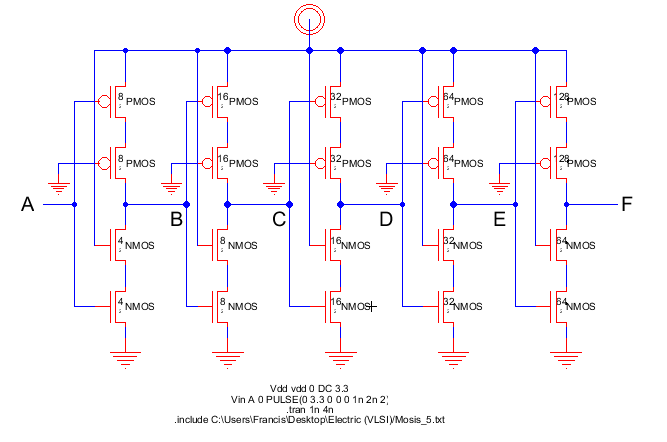
\includegraphics[scale=0.5]{./CircuitoFO2.png}
    \rule{35em}{0.5pt}
  \caption[Captura]{Circuito para calculo de $R_{eq}$ con h=2}
  \label{fig:CircuitoFO2}
  \end{center}
\end{figure}

\begin{figure}[htbp]
  \centering
    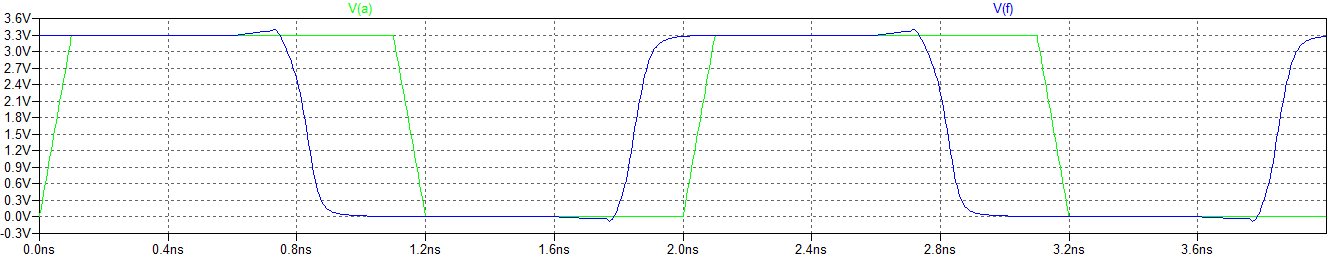
\includegraphics[scale=0.4]{./FO2.png}
    \rule{35em}{1pt}
  \caption[Captura]{Gráfica tiempo $V_{in}$ vs $V_{out}$ h=2}
  \label{fig:FO2}
\end{figure}

\begin{figure}[htbp]
\begin{center}
    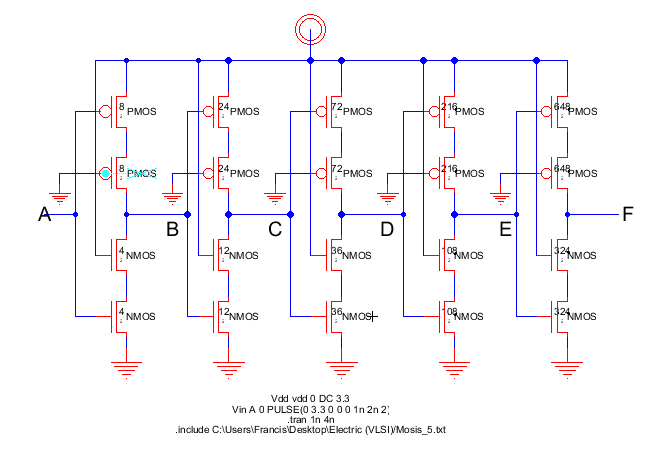
\includegraphics[scale=0.5]{./CircuitoFO3.png}
    \rule{35em}{0.5pt}
  \caption[Captura]{Circuito para calculo de $R_{eq}$ con h=3}
  \label{fig:CircuitoFO3}
  
\end{center}
\end{figure}

\begin{figure}[htbp]
  \begin{center}
    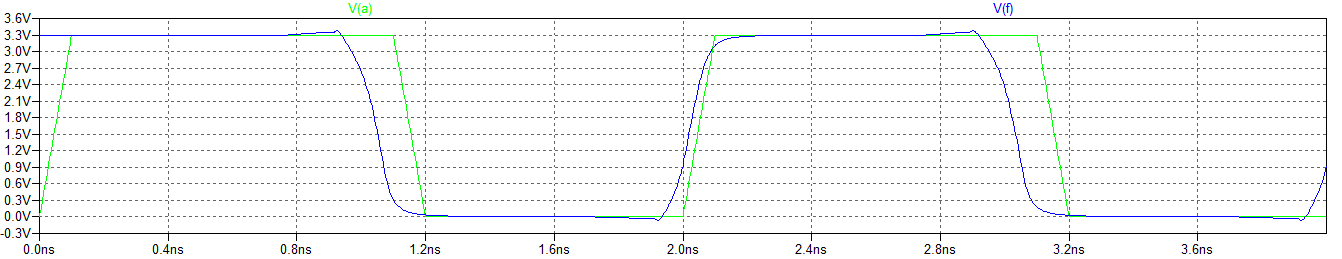
\includegraphics[scale=0.4]{./FO3.png}
    \rule{35em}{0.5pt}
  \caption[Captura]{Gráfica tiempo $V_{in}$ vs $V_{out}$ h=3}
  \label{fig:FO3}
  \end{center}
\end{figure}

Luego de encontrar las gráficas (fig. \ref{fig:FO2} y fig. \ref{fig:FO3}), se realizó la medición de los tiempos ya mencionados anteriormente. Aunque en la referencia [] se habla que la medición debe hacerse entre los valores de $0.8V_{dd}$ a $0.2V_{dd}$, se encontró que las pendientes de ambas graficas son aproximadamente iguales y no se encontraría la variación de la resistencia equivalente entre los CMOS por lo que se decidió medir de $0.9V_{dd}$ a $0.1V_{dd}$. Se encontraron los valores mencionados en el cuadro \ref{table:tiempos}. \\*
\\*
\begin{table}\label{table:tiempos}
\begin{center}
\begin{tabular}{c||c||c}
n & tr(ps) & tf(ps)\\
\hline
\hline
2 & 97.36 & 101.29 \\
3 & 117.84 & 125.055 \\
$\Delta$ & 20.44 & 23.76\\
\hline
\end{tabular}
\caption{Tiempos de levantamiento y caida de tensión para un inversor CMOS para diferentes Fanouts}
\end{center}
\end{table}


Ya con los diferenciales de tiempos medidos, se sustituyen en \ref{eqn:Req_p} y \ref{eqn:Req_n} para encontrar la resistencia equivalente de cada transistor. Para $C_{g}=1.48 fF/\mu m$  dependiente del ancho de canal de gate, se encuentra que los valores de resistencia son los del cuadro (\ref{table:resistencias}). \\*
\\*
\begin{table}\label{table:resistencias}
\begin{center}
\begin{tabular}{c||c}
Resistencia & k$\Omega$\\
\hline
\hline
$R_{eqp}$ & 15.375 \\
$R_{eqn}$ & 9.000 \\
\hline
\end{tabular}
\caption{Resistencias equivalentes encontradas por Método de Fanout}
\end{center}
\end{table}




\section{Análisis de datos y resultados.}

Los resultados obtenidos en la sección \textit{3.1.2}, muestran el diseño del ancho del canal de un transistor \textit{PMOS}, para conseguir que los tiempos de propagación sean simétricos. Los resultados obtenidos de la Ec.\ref{eqn:Beta2}, muestra un valor de relación de tamaño de ancho de canal de los transistores en un inversor de \textit{1.3070}, lo que equivale a decir que el ancho del canal del tansistor \textit{PMOS} es de 5$\lambda$, pero a la hora de simular se ajusto este valor hasta conseguir que la relación sea \textit{1.5}, esto con el fin no solo de lograr que los valores de propagación de la señal fueran simétricos, si no también para conseguir una tensión de umbral del inversor cercana a \textit{1.65V}, como se observa en la fig.\ref{fig:DC_Comp}, siendo asi entonces que el nuevo tamaño del ancho de canal del transistor \textit{PMOS} es de 6$\lambda$.\\*
\\*Uno de los resultados relevantes que pudimos encontrar del dimensionamiento del transistor \textit{PMOS} es en el hecho que las corrientes de corto circuito de la fig. \ref{fig:CC} son aproximadamente iguales, los cual nos dice que la potencia de los transistores en ambos procesos es igual. Podemos deducir que mediante un análisis dinámico para el dimensionamiento de los transistores es el método que deber usarse para el diseños de las compuertas, esto porque la símetría de las transiciones se puede obviar con respecto a tener un mínimo del tiempo de retardo para las mismas, dando como resultado, que los circuitos puedan conmutar a una mejor velocidad con la misma potencia que si se hiciese de forma simétrica las compuertas.\\*
\\*En la sección 3.2 se procede a calcular el valor de las resistencias de canal para un trasistror \textit{PMOS} y un transistor \textit{NMOS}, mediante dos métodos diferentes. \\

En la sección 3.2.1 se calculó la resistencia de canal por un método grafico, simulando la carga y descarga de un capacitor y obteniendo la curva de comportamiento de la corriente de \textit{drain} de un transistor \textit{PMOS} y \textit{NMOS}, respectivamente, y con esto obteniendo los valores de resistencia que se muestran en la Ec.\ref{eqn:R_PMOS} y Ec.\ref{eqn:R_NMOS}. Se considera que este método no es muy preciso al tratarse del cálculo de un valor a partir de una aproximación, que dependerá de la cantidad de valores muestrados y de la precisión de dichos valores, lo que dio como resultado obteniendo por ende un valor promedio de resistencia.\\*

En cambio, para la sección 3.2.2, encontramos que los valores de las resistencias equivalentes son mas precisos, por el método que se emplea y que no realiza tantas aproximaciones y suposiciones para encontrar el valor de los mismos.


\section{Conclusiones.}
\begin{itemize}
\item La ecuaciones de Shockley no da un comportamiento real de los transistores PMOS y NMOS, si no un comportamiento muy aproximado.
\item El uso de diversas herramientas de simulación nos permiten encontrar proporciones de diseño bastante precisas
\item El diseño de un inversor apropiado debe de procurar un balance entre el mejoramiento de los tiempos de propagación, asi como la obtención de una tension de umbral lo más cercana a $\textit{V}_\textit{DD}/2$.
\item El análisis de tiempos de propagación provee un mejor punto de arranque para la obtención del tamaño de un transistor \textit{PMOS}, permitiendo realizar ajustes en simulación que permitan llegar a un valor concreto de manera más rapida.
\item El método grafico para la obtención de los valores de resistencia de canal no es el mas apropiado, aunque provee una forma rapida de encontrar un valor de resistencia aproximado aceptable.
\item Se recomienda para encontrar la resistencia equivalente de los transistores el método de Fanout
\end{itemize}

%----------------------------------------------------------------------------------------
\begin{thebibliography}{3}

\bibliographystyle{unsrtnat} % Use the "unsrtnat" BibTeX style for formatting the Bibliography

\bibitem[Wey(1999)]{Wey1999}
[1] N. Weste, D. Harris. 
\newblock {CMOS VLSI Design: A Circuits and Systems Perspective , 4 edition.}.
\newblock \emph{Boston: Addison-Wesley}, 2010.

\bibitem[Wey(1999)]{Wey1999}
[2] J. Rabaey, A. Chandrakasan y B. Nikolic. 
\newblock { Digital Integrated Circuits: A Design Perspective.}.
\newblock \emph{Prentice Hall}, 2005.

\bibitem[Wey(1999)]{Wey1999}
[3]Test Data .On SemiconductorC5.Mosis. Recompilado de:
\newblock \emph{http://www.ie.itcr.ac.cr/achacon/ \\* Intro$\_$Diseno$\_$CI/Modelos$\_$Spice$\_$MOSIS/v03m-params.txt}, el 07/09/2015

\end{thebibliography}

\end{document}